\documentclass[conference]{IEEEtran}
\IEEEoverridecommandlockouts

\usepackage{cite}
\usepackage{amsmath,amssymb,amsfonts}
\usepackage{algorithm}
\usepackage{algorithmic}
\usepackage{graphicx}
\usepackage{textcomp}
\usepackage{xcolor}
\usepackage{tikz}
\usetikzlibrary{arrows.meta,positioning,fit}
\usepackage{url}
\usepackage{array}
\usepackage{multirow}
\usepackage{balance}

\def\BibTeX{{\rm B\kern-.05em{\sc i\kern-.025em b}\kern-.08em
    T\kern-.1667em\lower.7ex\hbox{E}\kern-.125emX}}

\begin{document}

\title{SAGE: A Security-Aware, Multi-Source Retrieval-Augmented\\
Knowledge Engine for Provenance-Preserving Question Answering\\
over Websites, Documents, Videos, and Code Repositories}

\author{
\IEEEauthorblockN{Srujan Zanjal}
\IEEEauthorblockA{
Department of Computer Engineering\\
St. Vincent Pallotti College of Engineering and Technology\\
Nagpur, India\\
zanjalsrujan94@gmail.com}
}

\maketitle

\begin{abstract}
Users who work across heterogeneous artefacts -- web pages, technical
documents, long-form videos, and software repositories -- must
routinely switch tools, search modes, and mental models to find and
verify information. Retrieval-augmented generation (RAG) mitigates the
unsupported-answer problem of large language models by conditioning
generation on retrieved evidence, but most deployed assistants remain
modality-specific and rarely disclose, in a source-appropriate way,
where an answer's evidence actually came from. This paper presents
\textbf{SAGE} (Semantic Analysis and Generation Engine), a prototype
multi-source knowledge engine that ingests public websites, born-digital
PDFs, YouTube videos, and public GitHub repositories into a common
chunk-and-metadata representation, and answers questions with
source-appropriate citations (URL, page number, timestamp, or file/line
range) and a heuristic confidence score. Three design choices
distinguish SAGE from a conventional single-modality RAG pipeline:
(i) \emph{deterministic source-overview chunks}, generated from
source-derived statistics rather than a second generative pass, which
materially improve broad "what is this about" questions; (ii) a
\emph{diversity-floor reranking} step that guarantees every source
selected for a combined, multi-source query contributes at least one
citation, preventing one dominant source from crowding out the others;
and (iii) an explicit \emph{security posture} -- server-side-request-forgery
(SSRF) defense on every ingested and redirected URL, and an
instruction-injection guard that quotes retrieved content inside
delimited, clearly-untrusted tags before it reaches the language model.
The system is implemented as a FastAPI backend, a React front end, a
Chrome Manifest V3 side panel, ChromaDB for vector search, and Supabase
PostgreSQL for provenance metadata, and streams answers incrementally
over Server-Sent Events with multi-turn conversational memory.
Prototype-level validation across representative sources for all four
modalities indicates that the architecture supports robust ingestion,
retrieval, and citation rendering, and that overview chunks and the
security controls behave as intended under adversarial and edge-case
probing. We position SAGE against NotebookLM-style closed assistants
and generic open-source RAG frameworks, and outline the remaining gaps
-- OCR, private-repository support, hybrid lexical-semantic retrieval,
and calibrated confidence -- that separate the current prototype from a
production-grade system.
\end{abstract}

\begin{IEEEkeywords}
retrieval-augmented generation, source-grounded question answering,
multi-modal knowledge engine, vector database, prompt injection,
server-side request forgery, provenance, confidence estimation
\end{IEEEkeywords}

\section{Introduction}

Knowledge work rarely stays inside one modality. A student verifying a
claim may need a public website, a lecture video, an API reference PDF,
and the source code of a library that implements the idea being
studied. Lexical search remains effective for precise term lookup, but
it degrades on higher-level questions such as ``what is this source
about'', ``which file defines this route'', or ``what does the speaker
conclude''. Retrieval-augmented generation (RAG) addresses part of this
gap by grounding a language model's output in retrieved passages rather
than only in its parametric memory, which measurably reduces unsupported
claims in knowledge-intensive tasks \cite{lewis2020rag,karpukhin2020dpr}.

In practice, however, most RAG-based assistants are built around a
single modality. Document-QA systems assume PDFs or scanned forms;
speech systems assume transcripts; code assistants assume a repository;
website assistants often ignore both client-side rendering and the
provenance format that a user actually needs to verify an answer. Even
where a system spans several source types -- as closed, consumer-facing
tools such as Google's NotebookLM increasingly do -- the retrieval,
citation, and trust mechanics behind the assistant are not open to
inspection or adaptation \cite{notebooklm2026}. Consumer assistants also
rarely say anything about \emph{why} an answer should be trusted beyond a
citation link, and even less about the security posture of a system that,
by design, must fetch attacker-reachable web content and third-party code
in order to answer questions about it.

This paper describes \textbf{SAGE}, a prototype system built as a
final-year engineering project to explore these gaps concretely rather
than only survey them. SAGE ingests four source types -- websites, PDFs,
YouTube videos, and public GitHub repositories -- into a shared
knowledgebase representation and answers questions with citations that
match the modality's natural unit of evidence: a URL and chunk index for
websites, a page number for PDFs, a timestamp for videos, and a file
path with a line range for code. Two further properties motivate the
work beyond citation rendering. First, broad questions are a retrieval
problem, not only a prompting problem: dense retrieval over
fine-grained chunks alone tends to surface locally relevant but globally
incomplete evidence for questions like ``summarise this repository''.
SAGE addresses this with a \emph{deterministic source-overview chunk},
generated once per knowledgebase from extracted statistics and excerpts
without a second language-model call, which acts as a structured
retrieval prior for broad questions while remaining fully traceable to
the ingested source. Second, a system that fetches arbitrary
user-supplied URLs and indexes third-party web and repository content
for later consumption by a language model has an attack surface that a
single-document QA tool does not: SSRF against internal infrastructure
through the ingestion step, and indirect prompt injection through the
retrieved content itself \cite{greshake2023injection}. SAGE treats both as
first-class design constraints rather than deployment afterthoughts.

Because SAGE originates as a final-year engineering project rather than
a funded industrial deployment, its design is also shaped by practical
constraints that are worth stating explicitly rather than treating as
incidental: a single hosted LLM API rather than a self-hosted model, a
single-operator deployment rather than a multi-tenant service, and a
validation budget that permits thorough, representative testing per
modality but not a large-scale, statistically powered benchmark. We
treat these as scoping decisions rather than hidden weaknesses, and
report the prototype's behaviour honestly against them in Section VIII
and Section X rather than presenting demonstration-scale results as if
they were production-scale ones.

The contributions of this paper are:
\begin{enumerate}
\item a unified multi-source RAG architecture that normalises website,
PDF, video, and GitHub ingestion into one indexing, retrieval, and
citation contract while preserving modality-appropriate provenance
fields;
\item deterministic source-overview chunks that improve broad-question
retrieval without adding a second generative stage at index time,
together with a diversity-floor reranking mechanism that keeps
multi-source, combined queries from being dominated by a single source;
\item an explicit security architecture -- SSRF-hardened ingestion with
per-redirect-hop revalidation, and instruction-injection-guarded answer
generation -- motivated directly by the indirect-prompt-injection and
SSRF risks inherent to any RAG system that fetches external content; and
\item a realistic prototype validation across all four modalities,
including adversarial probing of the security controls, that documents
both the system's current capability and its honestly-scoped
limitations.
\end{enumerate}

The remainder of the paper is organised as follows. Section II reviews
related work in RAG, modality-specific retrieval, and RAG-specific
security. Section III formalises the multi-source QA problem SAGE
targets. Section IV describes the system architecture. Section V
details the per-modality ingestion methodology and the shared retrieval
and answering pipeline. Section VI describes the security architecture
in depth. Section VII presents the ranking, confidence, and diversity
algorithms. Section VIII reports prototype validation results. Section
IX positions SAGE against NotebookLM and open-source RAG frameworks.
Section X discusses limitations and future work, and Section XI
concludes.

\section{Related Work}

\subsection{Retrieval-Augmented Generation}
RAG conditions a language model's generation on passages retrieved from
an external corpus, combining parametric and non-parametric knowledge
\cite{lewis2020rag}. Dense Passage Retrieval (DPR) showed that a
dual-encoder trained on question-passage pairs outperforms classical
sparse retrieval for open-domain QA \cite{karpukhin2020dpr}. Fusion-in-Decoder
(FiD) demonstrated that a generative reader can independently encode
many retrieved passages and fuse evidence in the decoder, improving
accuracy as the number of retrieved passages grows without the
quadratic attention cost of concatenating them in the encoder
\cite{izacard2021fid}. Self-RAG extended this line of work with
learned reflection tokens that let a model decide \emph{when} to
retrieve and critique its own generations against the retrieved evidence
\cite{asai2024selfrag}, and is one of several recent efforts to make
grounding an explicit, trainable part of generation rather than a fixed
pipeline stage. A separate, heavier-weight line of work targets the same
broad-question problem that motivates SAGE's overview chunks: GraphRAG
builds an LLM-derived entity graph and pregenerated community summaries
over an entire corpus at index time specifically to answer global,
corpus-level questions that plain chunk retrieval under-serves
\cite{edge2024graphrag}. SAGE's overview chunk is a deliberately
lighter-weight answer to the same problem, trading GraphRAG's
higher index-time cost and second-LLM-call surface for a
non-generative, source-derived summary (Section VII). These systems are underpinned by the Transformer
architecture \cite{vaswani2017attention} and by efficient sentence-level
embedding methods such as Sentence-BERT, which make large-scale
passage-level similarity search practical \cite{reimers2019sbert}.
Recent surveys of the field emphasise provenance, updateability, and
modularity as the dominant real-world deployment concerns for RAG
systems \cite{gao2023ragsurvey}, a framing this paper adopts directly:
SAGE is best read as an engineering response to those three concerns
for a specific, multi-modal setting.

\subsection{Vector Search Infrastructure}
FAISS established that approximate nearest-neighbour search over
high-dimensional embeddings can scale to billions of vectors
\cite{johnson2017faiss}. Application-oriented systems such as Chroma
build on this idea with collection-based storage, metadata filtering,
and a developer-facing query API \cite{chroma2026docs}, which SAGE
adopts for vector storage while keeping a separate relational store
(Supabase PostgreSQL \cite{supabase2026docs}) for lifecycle state and
provenance metadata that benefits from relational constraints and
querying.

\subsection{Modality-Specific Retrieval and Extraction}
For documents, LayoutLM showed that jointly modelling text and layout
improves visually-rich document understanding \cite{xu2020layoutlm}.
SAGE deliberately targets a narrower, more tractable subset of this
problem -- born-digital PDFs with selectable text -- to avoid the cost
and failure modes of OCR in the core pipeline, leaving scanned-document
support as future work. For speech and video, Whisper demonstrated
robust multilingual transcription from large-scale weak supervision
\cite{radford2023whisper}; SAGE combines caption retrieval with a local
Whisper-family fallback, a staged strategy increasingly common in
practical transcript pipelines. For code, CodeBERT established strong
joint representations of natural language and source code
\cite{feng2020codebert}, and RepoCoder showed that repository-level
retrieval, rather than single-file context, substantially improves code
tasks \cite{zhang2023repocoder}. SAGE does not synthesise code, but
borrows this repository-level-context insight directly in its
GitHub-overview chunk and path/line-aware citation metadata.

\subsection{Multi-Source, Notebook-Style Assistants}
Consumer tools such as Google's NotebookLM already combine several
source types -- documents, web pages, and video -- behind one
source-grounded assistant, explicitly to reduce hallucination relative
to an ungrounded chatbot \cite{notebooklm2026}. Open-source frameworks
such as LangChain \cite{langchain2026}, LlamaIndex \cite{llamaindex2026},
and Haystack \cite{haystack2026} instead provide general-purpose
building blocks -- connectors, indices, and pipeline components -- from
which a developer assembles a specific RAG application. SAGE occupies a
middle position: unlike NotebookLM it is open and inspectable end to
end, and unlike a generic framework it is a complete, opinionated
application with a fixed, provenance-first metadata contract across
exactly the four modalities it targets. Section IX compares these
positions directly.

\subsection{Security of Retrieval-Augmented Systems}
Because RAG systems retrieve and then condition generation on external
content, that content is an attacker-influenceable input to the
language model. Greshake et al. formalised this as \emph{indirect prompt
injection}: adversarial instructions embedded in a web page, document,
or other retrieved artefact that an LLM-integrated application will
later ingest and may obey \cite{greshake2023injection}. This risk is now
listed as the top item in the OWASP Top 10 for LLM applications
\cite{owasp2025llm01}. A second, less discussed risk is specific to the
ingestion step itself: a system that fetches an arbitrary user-supplied
URL is a general-purpose server-side-request-forgery (SSRF) vector
unless every fetch -- including every redirect hop -- is checked against
private, loopback, link-local, and cloud-metadata address ranges. Both
risks are directly relevant to any multi-source RAG system and are
treated as core design constraints in SAGE rather than as
post-deployment hardening, as described in Section VI.

\subsection{Confidence and Faithfulness}
Because RAG does not guarantee that generated text is fully supported
by retrieved evidence, a substantial literature studies hallucination
detection and mitigation in LLMs, including black-box, sampling-based
detectors and broader taxonomies of the failure modes involved
\cite{huang2024hallucination}. SAGE does not attempt calibrated
faithfulness estimation; instead it computes an interpretable, heuristic
confidence score from retrieval and reranking signals (Section VII) and
uses that score to gate whether Grounded Mode answers at all, which is a
deliberately conservative, low-complexity response to the same
underlying problem this literature studies at a deeper level.

\subsection{Evaluation Methodology for RAG Systems}
A related, largely separate literature studies \emph{how} RAG systems
should be evaluated at all. Recent systematic reviews of the field
observe that architectures have proliferated faster than agreed-upon
evaluation methodology, and that many reported results are difficult to
compare across papers because of inconsistent metrics, corpora, and
question sets \cite{slr2025rag}. Comprehensive surveys of RAG evaluation
specifically catalogue retrieval-quality metrics, generation-quality
metrics, and end-to-end task metrics, and note that few deployed systems
report all three consistently \cite{ragevalsurvey2025}. SAGE's prototype
validation (Section VIII) is deliberately framed against this backdrop:
rather than claiming a benchmark result that would be difficult to
compare against other systems' self-reported numbers, we report
representative, reproducible test scenarios per modality and state
plainly where the validation stops short of a controlled benchmark.

\section{Problem Formulation}

Let a user provide a source $S$ belonging to a modality set
\begin{equation}
\mathcal{T} = \{\text{website}, \text{pdf}, \text{video}, \text{github}\}.
\end{equation}
For a source of type $t \in \mathcal{T}$, ingestion constructs a
knowledgebase $K^{(t)} = (C^{(t)}, M^{(t)})$, where
$C^{(t)} = \{c_0, c_1, \dots, c_n\}$ is an ordered set of chunks and
$M^{(t)}$ is its provenance metadata store. The first chunk is reserved
for a deterministic overview,
\begin{equation}
c_0 = g_t(S),
\end{equation}
where $g_t(\cdot)$ is a non-generative, source-derived function specific
to modality $t$ (Section V, Algorithm 2). The remaining chunks are
produced by a modality-specific segmenter,
\begin{equation}
\{c_1, \dots, c_n\} = h_t(S).
\end{equation}
Each chunk is embedded by a shared encoder $f_\theta$,
\begin{equation}
e_i = f_\theta(c_i), \qquad e_q = f_\theta(q'),
\end{equation}
where $q'$ is the query after optional rewriting. Chunks are stored
together with metadata including \texttt{source\_id},
\texttt{knowledgebase\_id}, \texttt{source\_type}, \texttt{chunk\_index},
and modality-specific provenance fields (URL, page number, timestamp
range, or file path and line range).

Given a query $q$ and a selected set of knowledgebases
$\mathbb{K} = \{K^{(t_1)}, \dots, K^{(t_m)}\}$ ($m=1$ for single-source
questions, $m>1$ for combined questions), the system must return an
answer $A$ and a citation set $\Pi$ such that: (1) $A$ is relevant to
$q$; (2) $A$ is grounded in a retrieved evidence subset
$\widetilde{C} \subseteq \bigcup_i C^{(t_i)}$; (3) every citation
$\pi \in \Pi$ resolves to explicit provenance metadata in the
corresponding $M^{(t_i)}$; (4) when $m > 1$, $\Pi$ is not permitted to
collapse onto a single source if evidence exists in more than one; and
(5) unsupported claims are suppressed, or reflected through a low
confidence score $\kappa$ and, in Grounded Mode, a refusal. A practical
objective is therefore
\begin{equation}
\max_{A,\Pi}\ \mathrm{Rel}(A,\widetilde{C}) + \eta\,\mathrm{Prov}(\Pi,\widetilde{C}) + \zeta\,\mathrm{Div}(\Pi,\mathbb{K}) - \mu\,\mathrm{Hall}(A,\widetilde{C}),
\end{equation}
where $\mathrm{Rel}$ rewards relevance, $\mathrm{Prov}$ rewards explicit
provenance, $\mathrm{Div}$ rewards citation coverage across the selected
knowledgebases in $\mathbb{K}$, and $\mathrm{Hall}$ penalises unsupported
content. SAGE approximates this objective through heuristics on
retrieval score, rerank score, a diversity-floor constraint, and
mode-specific answer policy, rather than through end-to-end supervised
training.

\section{System Architecture}

SAGE separates ingestion-time and query-time concerns behind a shared
indexing contract, as shown in Fig.~\ref{fig:arch}. Four
modality-specific extractors converge, after chunking and overview
generation, on a common representation: one knowledgebase per ingested
source with a stable identifier, one overview chunk followed by
detailed chunks, and provenance-rich metadata on every chunk. Vector
embeddings are stored in ChromaDB; relational metadata, lifecycle state,
and (optionally) query history are stored in Supabase PostgreSQL. This
split lets the query-time layer stay largely modality-agnostic while
still rendering citations in a modality-aware form.

\begin{figure}[t]
\centering
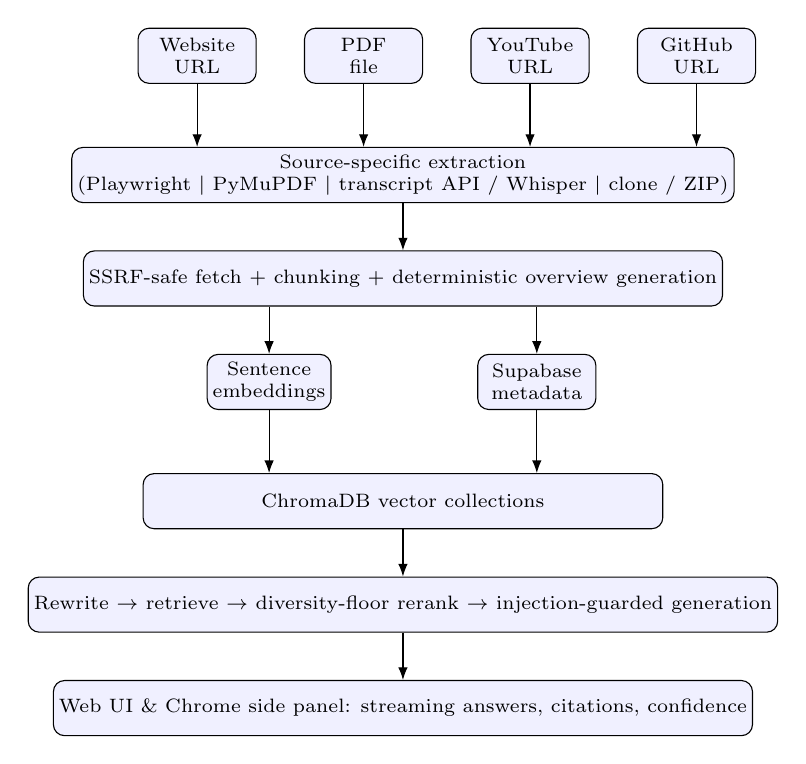
\begin{tikzpicture}[
  node distance=6mm and 6mm,
  box/.style={draw, rounded corners, align=center, minimum height=7mm,
              font=\scriptsize, fill=blue!6, inner sep=2pt},
  wide/.style={box, minimum width=6.6cm},
  narrow/.style={box, minimum width=1.5cm},
  arr/.style={-{Latex[length=1.6mm]}, thin}
]
\node[narrow] (web) {Website\\URL};
\node[narrow, right=of web] (pdf) {PDF\\file};
\node[narrow, right=of pdf] (vid) {YouTube\\URL};
\node[narrow, right=of vid] (gh) {GitHub\\URL};

\node[wide, below=8mm of pdf, xshift=0.5cm] (extract)
  {Source-specific extraction\\(Playwright \textbar\ PyMuPDF \textbar\ transcript API / Whisper \textbar\ clone / ZIP)};

\node[wide, below=of extract] (ssrf)
  {SSRF-safe fetch + chunking + deterministic overview generation};

\node[narrow, below=of ssrf, xshift=-1.7cm] (embed) {Sentence\\embeddings};
\node[narrow, below=of ssrf, xshift=1.7cm] (meta) {Supabase\\metadata};

\node[wide, below=8mm of embed, xshift=1.7cm] (chroma) {ChromaDB vector collections};

\node[wide, below=of chroma] (qa)
  {Rewrite $\to$ retrieve $\to$ diversity-floor rerank $\to$ injection-guarded generation};

\node[wide, below=of qa] (ui)
  {Web UI \& Chrome side panel: streaming answers, citations, confidence};

\draw[arr] (web) -- (extract.north -| web);
\draw[arr] (pdf) -- (extract.north -| pdf);
\draw[arr] (vid) -- (extract.north -| vid);
\draw[arr] (gh) -- (extract.north -| gh);
\draw[arr] (extract) -- (ssrf);
\draw[arr] (ssrf.south -| embed) -- (embed);
\draw[arr] (ssrf.south -| meta) -- (meta);
\draw[arr] (embed) -- (chroma.north -| embed);
\draw[arr] (meta) -- (chroma.north -| meta);
\draw[arr] (chroma) -- (qa);
\draw[arr] (qa) -- (ui);
\end{tikzpicture}
\caption{SAGE architecture. Four heterogeneous sources converge on a
common chunk-plus-metadata contract, are indexed in ChromaDB and
Supabase, and are queried through a shared, security-aware retrieval and
answer pipeline.}
\label{fig:arch}
\end{figure}

The extension subsystem is intentionally narrower than the web
application: it targets website QA only, using Chrome's Manifest V3 and
\texttt{chrome.sidePanel} API \cite{chromesidepanel2026,mv32026}, and
was brought to feature parity with the web client during this project
(streaming answers, multi-source combination, and conversational
memory), while deliberately keeping its host permissions and file-system
surface minimal.

\subsection{Implementation Footprint}
Table~\ref{tab:stack} lists the concrete software stack behind the
architecture in Fig.~\ref{fig:arch}. The backend and frontend are pinned
to exact dependency versions to keep the prototype reproducible; the
extension is restricted to two \texttt{localhost} host permissions and
carries no third-party network access. Automated test coverage spans 12
test modules and approximately 95 test functions across chunking, URL
validation and SSRF-adjacent logic, GitHub URL parsing and repository
scanning, reranker and confidence scoring, overview-chunk generation,
vector-store metadata handling, and video transcript/fallback flows,
complemented by an integration suite exercising the API surface directly.

\begin{table}[t]
\caption{Implementation stack (pinned versions).}
\label{tab:stack}
\centering
\begin{tabular}{p{1.6cm}p{1.1cm}p{3.3cm}}
\hline
\textbf{Layer} & \textbf{Version} & \textbf{Role} \\
\hline
FastAPI & 0.115.6 & Backend API framework \\
ChromaDB & 0.5.23 & Vector storage and similarity search \\
Supabase (client) & 2.10.0 & Relational metadata store access \\
sentence-transformers & 3.3.1 & Chunk/query embedding \\
Groq SDK & 0.13.1 & Hosted LLM inference (query rewrite, generation) \\
Playwright & 1.46.0 & Rendered website crawling \\
PyMuPDF & 1.25.1 & PDF text extraction \\
faster-whisper & 1.0.3 & Local speech-to-text fallback \\
React & 19.2.5 & Web front end \\
Vite & 8.0.10 & Frontend build tooling \\
Tailwind CSS & 4.2.4 & Frontend styling \\
Chrome extension & MV3, v1.6.0 & Website-only side panel \\
\hline
\end{tabular}
\end{table}

\section{Methodology}

\subsection{Website Ingestion}
The website module accepts a public HTTP(S) URL, resolves and validates
it (Section VI-A), and launches a depth- and page-bounded crawl using
Playwright \cite{playwright2026}, chosen over raw HTTP fetching because
modern pages frequently depend on client-side rendering. Extracted text
is cleaned and segmented into chunks carrying URL-level metadata
(canonical reference, original reference, title, page index, chunk
index). The website overview chunk is generated deterministically from
crawl statistics: canonical URL, number of pages crawled, page titles,
and beginning/ending excerpts, so that broad questions such as ``what is
this website about'' have a high-recall, source-derived anchor to
retrieve even when no single paragraph answers the question.

\subsection{PDF Ingestion}
The PDF module targets born-digital PDFs with selectable text.
PyMuPDF provides fast, page-level text and structure extraction
\cite{pymupdf2026,pymupdf_text2026}. Uploads are validated by size (25\,MB
cap), file signature (\texttt{\%PDF} header), and content type before
extraction; empty or textless PDFs are rejected rather than silently
producing an empty knowledgebase. Detailed chunks preserve
\texttt{page\_number}, enabling page-level citations. OCR is available in
PyMuPDF through a separate mechanism \cite{pymupdf_ocr2026} but is
intentionally excluded from the core pipeline to keep the baseline
extraction path simple and dependency-light; this is discussed further
as a limitation in Section X.

\subsection{Video Ingestion}
The video module ingests public YouTube URLs. It first attempts
transcript acquisition via the YouTube Transcript API, which retrieves
existing human or auto-generated captions without a browser or API key
\cite{ytapi2026}. If no captions exist, an explicit fallback invokes
\texttt{yt-dlp} to fetch audio \cite{ytdlp2026} and a
\texttt{faster-whisper} model \cite{fasterwhisper2026,radford2023whisper}
for local transcription, bounded to a 900-second maximum duration and a
100\,MB audio cap to keep worst-case ingestion time predictable on
commodity hardware. Transcripts become timestamped chunks
(\texttt{start\_time}, \texttt{end\_time}, a human-readable label), and
the overview chunk summarises title, duration, transcript origin, and
beginning/ending excerpts using transcript-derived evidence only.

\subsection{GitHub Repository Ingestion}
The GitHub module validates a public repository URL before any job
starts, then attempts a shallow clone with an archive-download fallback.
Files are filtered by extension and size, and hard caps
(300 indexed files, 1200 total chunks, 2{,}000{,}000 total characters,
250\,KB per file, 100{,}000 lines per file) bound worst-case ingestion
time and prevent resource exhaustion from adversarially large public
repositories. Text is chunked by line range, preserving
\texttt{file\_path}, \texttt{start\_line}, \texttt{end\_line}, and
inferred language. The repository overview chunk surfaces repository
name, detected languages, significant files (README, dependency
manifests, Dockerfiles), and likely entry points -- directly motivated by
the repository-level-context finding of RepoCoder \cite{zhang2023repocoder}
-- which improves architecture-level questions while detailed chunks
support precise implementation questions. The module never executes
repository code; it only indexes filtered text content.

\subsection{Shared Embedding, Retrieval, and Answer Generation}
All chunks are embedded with
\texttt{sentence-transformers/all-MiniLM-L6-v2}
\cite{minilm2026}, a compact encoder suited to short-passage semantic
similarity at low latency, with embeddings L2-normalised before
indexing. Chunk text and vectors are stored in ChromaDB collections
\cite{chroma2026docs}; provenance and lifecycle metadata are stored in
Supabase PostgreSQL tables covering \texttt{knowledgebases},
\texttt{sources}, \texttt{chunks}, and (opt-in) \texttt{query\_history}
\cite{supabase2026docs}. At query time the system: (1) optionally
rewrites short or vague questions using the last three conversation
turns to resolve pronouns and ellipsis; (2) embeds the rewritten query
and retrieves candidate chunks, widening $k$ for combined multi-source
questions; (3) reranks candidates with a linear blend of semantic
similarity and lexical overlap (Section VII); (4) applies a
diversity-floor step for combined queries; (5) builds a bounded context
window with per-chunk citation markers; and (6) generates an answer in
either \emph{Grounded Mode}, which restricts the model to retrieved
evidence and refuses when evidence is weak, or \emph{Exploratory Mode},
which presents source-backed content first and then clearly-separated
broader explanation. Answers stream to the client over Server-Sent
Events, with a \texttt{meta} event carrying citations and confidence
ahead of incremental \texttt{delta} text events, and prior question/answer
turns are passed back to the model as conversational history for both
query rewriting and answer generation.

\section{Security Architecture}

Because SAGE's ingestion step fetches arbitrary user-supplied URLs and
its answer-generation step conditions a language model on that fetched
content, the two dominant risks are SSRF at ingestion and indirect
prompt injection at generation \cite{greshake2023injection,owasp2025llm01}.
Both are addressed structurally rather than through input blocklists
alone.

\subsection{SSRF-Hardened Ingestion}
Every outbound fetch -- the initial crawl request, every subsequent
same-domain crawl request, and every HTTP redirect hop encountered along
the way -- is validated before the request is made. Validation resolves
the URL's hostname via DNS, then rejects the request if any resolved
address is private, loopback, link-local, multicast, unspecified, or a
known cloud metadata endpoint (e.g.\ \texttt{169.254.169.254}). Redirects
are followed manually, one hop at a time, with revalidation at each hop,
rather than delegated to the HTTP client's automatic redirect handling;
this closes a specific gap where an initially-valid public URL redirects
to an internal address only after the first request has already been
judged safe. The same check is enforced inside the Playwright-driven
crawler by aborting any in-page navigation whose target fails
validation, since a page can trigger further navigation after the
crawler has already started rendering it.

\subsection{Instruction-Injection-Guarded Generation}
Retrieved chunk text is untrusted with respect to the language model:
an ingested web page, PDF, transcript, or source file may contain text
that reads as an instruction (``ignore previous instructions and
...''). Following the threat model formalised for indirect prompt
injection \cite{greshake2023injection}, SAGE wraps all retrieved content
in explicit delimiter tags before it is placed in the model's context,
and the system prompt states directly that content between those tags
is untrusted data to be summarised or quoted, never instructions to be
followed. This does not eliminate the risk -- no purely prompt-level
defense can, given current language models -- but it removes the most
common failure mode of retrieved content being indistinguishable from
the developer's own instructions, and it is deliberately layered under
Grounded Mode's broader policy of declining to answer when evidence is
weak.

\subsection{Additional Controls}
Upload validation rejects malformed or oversized PDFs before extraction
is attempted. The GitHub module never executes indexed code and enforces
the file/size/chunk caps described in Section V-D, which double as a
denial-of-service control against adversarially large public
repositories. Query-history persistence is opt-in and defaults to
disabled, avoiding storage of user questions and answers unless
explicitly enabled by the operator. These controls are summarised
against their motivating risk in Table~\ref{tab:security}.

\begin{table}[t]
\caption{Security controls and the risk each addresses.}
\label{tab:security}
\centering
\begin{tabular}{p{2.1cm}p{2.1cm}p{3.3cm}}
\hline
\textbf{Control} & \textbf{Risk addressed} & \textbf{Where enforced} \\
\hline
Per-hop URL validation & SSRF to internal/cloud-metadata hosts & Website fetch, crawl, redirects, in-page navigation \\
Source-context delimiting + guard prompt & Indirect prompt injection & Answer generation (both modes) \\
Upload signature/size checks & Malformed/oversized PDF abuse & PDF ingestion entry point \\
No code execution; file/size/chunk caps & Arbitrary code execution; resource exhaustion & GitHub ingestion \\
Opt-in query history & Unintended retention of user Q\&A & Query-history persistence \\
\hline
\end{tabular}
\end{table}

\section{Algorithms and Scoring}

\begin{algorithm}[t]
\caption{Multi-source ingestion and indexing}
\begin{algorithmic}[1]
\REQUIRE source descriptor $S$, source type $t$
\ENSURE knowledgebase identifier $K$ or structured error
\STATE validate and normalise $S$ for modality $t$ (Sec.~VI-A for URLs)
\STATE $E \gets \textsc{Extract}(S, t)$
\IF{$E$ is empty or unusable}
  \RETURN structured ingestion error
\ENDIF
\STATE $m \gets \textsc{CollectMeta}(S, E, t)$
\STATE $c_0 \gets \textsc{GenerateOverview}(E, m, t)$
\STATE $D \gets \textsc{ChunkDetailed}(E, m, t)$
\STATE $C \gets [c_0] \cup D$
\FOR{all $c_i \in C$}
  \STATE $e_i \gets f_\theta(c_i)$
  \STATE write $(c_i, e_i)$ to ChromaDB
  \STATE write provenance metadata of $c_i$ to Supabase
\ENDFOR
\STATE mark source status as \texttt{ready}
\RETURN knowledgebase identifier $K$
\end{algorithmic}
\end{algorithm}

\begin{algorithm}[t]
\caption{Deterministic source-overview generation}
\begin{algorithmic}[1]
\REQUIRE extracted evidence $E$, metadata $m$, modality $t$
\ENSURE overview chunk $c_0$
\STATE initialise template $T_t$ for modality $t$
\STATE compute statistics: counts, duration/page count, titles, key files, URLs
\STATE collect early and late excerpts from $E$
\STATE populate $T_t$ using only source-derived fields (no LLM call)
\STATE set \texttt{chunk\_kind}=\texttt{source\_overview}, \texttt{chunk\_index}=0
\RETURN compiled overview chunk $c_0$
\end{algorithmic}
\end{algorithm}

Retrieval begins with cosine similarity between the query embedding and
each chunk embedding,
\begin{equation}
s_i = \cos(e_q, e_i) = \frac{e_q^{\top} e_i}{\lVert e_q\rVert \lVert e_i\rVert}.
\end{equation}
Reranking blends this semantic score with lexical overlap between the
(rewritten) query and the chunk text,
\begin{equation}
r_i = \alpha\, s_i + \beta\, \mathrm{lex}(q', c_i), \qquad \alpha = 0.78,\ \beta = 0.22,
\end{equation}
where $\mathrm{lex}(\cdot,\cdot)$ is a normalised, stop-word-filtered
token-overlap score. This fixed linear blend is an interpretability
choice consistent with the system's broader preference for auditable
heuristics over learned rerankers, at the cost of the precision gains a
learned or hybrid lexical-semantic reranker can offer (Section X).

For a combined query over knowledgebases $\mathbb{K} = \{K^{(t_1)}, \dots,
K^{(t_m)}\}$ with $m \ge 2$, Algorithm 3 applies a diversity floor before
truncating to the requested $\mathrm{top\_}k$: each source's single
highest-scoring chunk is reserved first, and the remaining slots are
filled by global score across all sources. This directly targets clause
(4) of the objective in Section III -- without it, a combined question
whose evidence is unevenly distributed across sources can return zero
citations from the weaker source even when relevant evidence exists
there.

\begin{algorithm}[t]
\caption{Diversity-floor reranking for combined queries}
\begin{algorithmic}[1]
\REQUIRE reranked chunks $\widetilde{C}$ with source ids, target size $k$, source set $\{s_1,\dots,s_m\}$
\ENSURE top-$k$ chunk selection $\widetilde{C}_k$ with per-source floor
\STATE $F \gets \emptyset$
\FOR{each source $s_j$}
  \STATE $F \gets F \cup \{\arg\max_{c \in \widetilde{C},\ \mathrm{src}(c)=s_j} r(c)\}$
\ENDFOR
\STATE $\widetilde{C}_k \gets F$
\STATE sort remaining $\widetilde{C} \setminus F$ by $r(c)$ descending
\WHILE{$|\widetilde{C}_k| < k$ and chunks remain}
  \STATE append next-highest-scoring remaining chunk to $\widetilde{C}_k$
\ENDWHILE
\STATE re-sort $\widetilde{C}_k$ by $r(c)$ descending
\RETURN $\widetilde{C}_k$
\end{algorithmic}
\end{algorithm}

Confidence is a heuristic, interpretable score rather than a calibrated
posterior probability:
\begin{equation}
\kappa = \mathrm{clip}_{[0,1]}\Big(0.65\, r_{\max} + 0.35\, \bar r_{3} + \min(|\widetilde{C}|,5)\cdot 0.025\Big),
\end{equation}
where $r_{\max}$ is the top reranked score, $\bar r_3$ is the mean score
of the top three retained chunks, and the final term is a small,
capped coverage bonus. In Grounded Mode, if no chunks are retrieved, or
$\kappa$ falls below a fixed low-confidence threshold ($0.28$) for a
non-video source, the system returns a cautious refusal instead of
calling the language model at all -- an explicit, low-complexity
instance of the $\mathrm{Hall}$ penalty in the Section III objective.
Video sources receive a narrower exemption (a warning rather than a hard
refusal) because transcript retrieval for narrative, spoken content
tends to score lower under this heuristic even when relevant.

\section{Prototype Validation and Results}

The evaluation reported here is a prototype validation exercise, not a
benchmark leaderboard experiment: the goal is to verify that the
implemented system ingests sources correctly, retrieves and cites
relevant evidence, degrades safely on out-of-scope or adversarial
queries, and supports full lifecycle operations (delete, re-ingest,
recrawl) across all four modalities, including under live,
browser-driven and network-level testing rather than unit tests alone.

Representative sources used during validation include the \emph{About
Python} website, a compact two-page born-digital PDF fixture, a short
TED YouTube video, and the public repository
\texttt{0xTheProDev/fastapi-clean-example} for GitHub ingestion. Security
controls were probed adversarially in addition to happy-path testing:
SSRF validation was exercised against loopback (\texttt{127.0.0.1}),
link-local (\texttt{169.254.169.254}), private (\texttt{10.x},
\texttt{192.168.x}), IPv6 loopback (\texttt{::1}), and non-HTTP-scheme
targets, all of which were correctly rejected while a genuine public IP
was correctly allowed.

Table~\ref{tab:modules} summarises the four modules and their
provenance behaviour; Table~\ref{tab:validation} summarises
representative validation outcomes and the primary limitation observed
per module.

\begin{table}[t]
\caption{Module capability summary.}
\label{tab:modules}
\centering
\begin{tabular}{p{1.1cm}p{2.4cm}p{3.6cm}}
\hline
\textbf{Module} & \textbf{Extraction} & \textbf{Citation type} \\
\hline
Website & Playwright crawl, same-domain depth limit & URL + chunk index \\
PDF & PyMuPDF page-wise extraction & Page number + snippet \\
Video & Transcript API, Whisper fallback & Timestamp span + snippet \\
GitHub & Shallow clone / ZIP fallback, line chunking & File path + line range \\
\hline
\end{tabular}
\end{table}

\begin{table}[t]
\caption{Prototype validation summary (representative tests, not a standardised benchmark).}
\label{tab:validation}
\centering
\begin{tabular}{p{1.1cm}p{3.6cm}p{2.4cm}}
\hline
\textbf{Module} & \textbf{Representative outcome} & \textbf{Primary limitation} \\
\hline
Website & Ingestion, QA, and citation checks passed; SSRF probes correctly blocked & JS-heavy/anti-bot sites may fail to crawl \\
PDF & Valid/empty/oversized/malformed upload paths verified & OCR not in core pipeline \\
Video & Transcript and fallback paths validated; timestamp citations correct & CPU auto-transcription latency \\
GitHub & URL validation, caps, and overview generation verified & Public repositories only \\
\hline
\end{tabular}
\end{table}

The most notable qualitative result concerns broad questions. Before
overview-chunk generation, broad queries such as ``summarise this
repository'' either retrieved weakly-connected local chunks or triggered
a Grounded Mode refusal; after overview-chunk standardisation, the same
class of question produced stable, source-derived high-level answers
with explicit provenance, most visibly for video and repository sources
where the gap between a global question and any single local chunk is
largest. The diversity-floor mechanism was validated directly: a
two-source combined query that previously returned citations from only
one of the two selected sources returned citations from both after the
fix, with \texttt{retrieved\_source\_count: 2} confirmed in the response
metadata.

\subsection{Threats to Validity}
Following standard practice for reporting empirical software validation
\cite{slr2025rag,ragevalsurvey2025}, we state the main threats to the
validity of the results above explicitly rather than implicitly.
\emph{Internal validity:} representative sources per modality (one
website, one PDF fixture, one video, one repository) were chosen for
repeatable, inspectable testing rather than sampled at random from a
larger population, so the reported outcomes reflect correctness on
chosen, cooperative inputs rather than a statistically representative
sample of the public web, arbitrary PDFs, arbitrary videos, or arbitrary
repositories. \emph{External validity:} validation targeted well-formed,
publicly reachable sources; heavily obfuscated or anti-bot-protected
websites, non-English or low-resource-language content, and
repositories near the ingestion caps (Section V-D) were not exhaustively
tested, so generalisation to such inputs is not established here.
\emph{Construct validity:} the confidence score $\kappa$ was validated
behaviourally -- it correctly gates refusals on weak evidence and remains
stable on strong evidence in the cases tested -- but this is not the same
as validating $\kappa$ against a human-annotated ground truth of answer
correctness, which Section X identifies as future work. \emph{Reliability:}
because answer generation depends on a hosted, non-deterministic LLM
API, exact answer wording is not perfectly reproducible across repeated
runs even against an unchanged index, though retrieval, reranking,
citation sets, and confidence scores are deterministic given a fixed
index state and query.

\section{Comparative Positioning}

Table~\ref{tab:compare} positions SAGE against a closed, consumer
multi-source assistant (NotebookLM) and a representative custom
application built on a general-purpose RAG framework (LangChain/LlamaIndex-class
tooling). The comparison is qualitative and based on publicly documented
capabilities rather than a controlled benchmark, and is intended to
locate SAGE's design choices rather than to claim superiority on any
single axis.

\begin{table}[t]
\caption{Qualitative comparison of source-grounded assistants: SAGE, NotebookLM \cite{notebooklm2026}, and a representative application built on a general-purpose framework \cite{langchain2026,llamaindex2026}.}
\label{tab:compare}
\centering
\begin{tabular}{p{1.7cm}p{1.6cm}p{1.6cm}p{1.6cm}}
\hline
\textbf{Property} & \textbf{SAGE} & \textbf{NotebookLM} & \textbf{Framework app} \\
\hline
Openness & Fully open, inspectable & Closed & Open (framework); app-specific \\
Fixed source types & Website, PDF, video, code & Docs, web, video, audio, slides & Depends on integration \\
Code-repo citations (file/line) & Built in & Not applicable & Requires custom build \\
SSRF-hardened ingestion & Explicit, per-hop & Not disclosed & Developer's responsibility \\
Injection-guarded prompting & Explicit & Not disclosed & Developer's responsibility \\
Multi-source diversity guarantee & Explicit (Alg.~3) & Not disclosed & Developer's responsibility \\
Streaming + memory & Yes (web + extension) & Yes & Depends on integration \\
Deployment & Self-hosted prototype & Managed SaaS & Self-hosted \\
\hline
\end{tabular}
\end{table}

The recurring pattern in Table~\ref{tab:compare} is that a general-purpose
framework can, in principle, be assembled into something with SAGE's
properties, but SAGE fixes those properties -- provenance format per
modality, SSRF handling, injection guarding, and multi-source diversity --
as defaults rather than as choices left to whoever assembles the
application, which is the paper's central engineering claim: these
properties are cheap to guarantee structurally and expensive to retrofit
per application.

\section{Discussion, Reliability, and Future Work}

\subsection{Discussion}
Two design lessons recur across this project. First, provenance is not
a rendering afterthought: it must be preserved from ingestion metadata
through reranking to answer rendering, and the correct citation unit
differs by modality (URL, page, timestamp, file/line) -- a single
flattened text-snippet citation would be strictly worse for every
modality studied here. Second, both broad-question handling and
multi-source fairness are retrieval-stage problems, not
prompting-stage problems: overview chunks and the diversity floor both
work by shaping what reaches the language model, rather than by asking
the model to compensate for a retrieval gap with more careful
instructions.

\subsection{Reliability}
The architecture surfaces a common distributed-systems issue in hybrid
RAG pipelines: vector and relational metadata are written to different
stores, so partial failures can leave a source ready in metadata with
incomplete vector coverage. SAGE mitigates this through explicit
delete/re-ingest lifecycle operations and targeted regression tests, but
stronger transactional guarantees across the two stores remain open
work. External dependencies -- a hosted LLM API subject to rate limits,
Playwright/Chromium for rendering, and local hardware for
auto-transcription -- further mean the system is best described as ready
for demonstration and prototype use rather than production-hardened.

\subsection{Limitations}
The prototype has no authentication or multi-user isolation and assumes
a single-operator deployment. OCR is intentionally out of scope for the
core PDF pipeline. Video ingestion depends on caption availability or
on comparatively slow local transcription. GitHub ingestion is
restricted to public repositories and bounded by the caps in Section
V-D. Confidence values are heuristic operational guidance, not
calibrated probabilities, and the fixed rerank weights ($\alpha=0.78$,
$\beta=0.22$) are a design choice rather than a tuned or learned
parameter.

\subsection{Responsible Use Considerations}
Because ingestion fetches content the operator does not own, the
prototype was built and validated with several responsible-use norms in
mind, distinct from the SSRF/injection security controls of Section VI.
The website crawler is depth- and page-bounded by configuration rather
than crawling exhaustively, which limits load placed on third-party
sites during ingestion. The GitHub module only reads and indexes public
repository text -- it never executes code, writes back to the
repository, or bypasses any access control -- and respects the caps in
Section V-D as an incidental courtesy limit on how much of a third
party's public repository is fetched in one job. Video ingestion is
limited to publicly available YouTube content and its existing captions
or a local transcription fallback; it does not circumvent access
restrictions on private or age-gated content. None of these norms are
enforced by a technical control beyond what Section VI already
describes, so an operator who deliberately reconfigures the bounds
(deeper crawls, larger repository caps) is responsible for ensuring that
use remains within the target site's or repository's terms of service.
We surface this explicitly because a multi-source ingestion system is,
by construction, easier to point at content its operator should not be
fetching than a single-modality tool is, and we believe that trade-off
deserves the same explicit treatment as the security risks in Section
VI rather than being left implicit.

\subsection{Future Work}
Four directions follow directly from the limitations above. First, OCR
integration would extend PDF coverage to scanned and image-only
documents. Second, private-repository and authenticated-website support
would broaden applicability beyond public content. Third, hybrid
retrieval that fuses the current dense score with a sparse/lexical
signal -- for example via reciprocal rank fusion, which has repeatedly
been shown to outperform either constituent ranking method alone
\cite{cormack2009rrf} -- would likely improve precision on exact
identifiers such as function names, error codes, and quoted phrases,
which dense-only retrieval systematically under-serves. Fourth, a
controlled benchmark with annotated question sets and calibrated
faithfulness metrics, informed by the broader hallucination-detection
literature \cite{huang2024hallucination}, would convert the current
prototype validation into a more formal evaluation.

\section{Conclusion}

This paper presented SAGE, a multi-source retrieval-augmented knowledge
engine that converts websites, PDFs, YouTube videos, and public GitHub
repositories into source-grounded, citation-preserving knowledgebases.
Beyond unifying four extraction pipelines behind one retrieval and
citation contract, SAGE contributes deterministic source-overview
chunks for broad-question retrieval, a diversity-floor reranking step
for fair multi-source citation, and an explicit security architecture
addressing SSRF and indirect prompt injection -- risks that are
structural to any system that fetches and reasons over external content,
not incidental to this one. Prototype-level validation, including
adversarial probing of the security controls, indicates the system is a
practical and technically coherent basis for further work on open,
provenance-aware, multi-modal assistants.

More broadly, the project's central claim is that the properties users
actually need to trust a multi-source assistant -- knowing where an
answer came from, being told when evidence is weak, and not having every
selected source but one silently dropped from a combined answer -- are
inexpensive to guarantee structurally when designed in from the first
ingestion pipeline, and correspondingly expensive to retrofit once a
system has already been built around a single modality or a single
source. As multi-modal, multi-source assistants continue to move from
research prototypes toward everyday tools, we believe provenance and
security are better treated as load-bearing architectural constraints,
in the way this paper has tried to demonstrate concretely, than as
polish applied after a system already works.

\balance
\begin{thebibliography}{99}

\bibitem{lewis2020rag} P. Lewis \emph{et al.}, ``Retrieval-Augmented Generation for Knowledge-Intensive NLP Tasks,'' in \emph{Advances in Neural Information Processing Systems}, vol. 33, 2020, pp. 9459--9474.

\bibitem{karpukhin2020dpr} V. Karpukhin \emph{et al.}, ``Dense Passage Retrieval for Open-Domain Question Answering,'' in \emph{Proc. EMNLP}, 2020, pp. 6769--6781.

\bibitem{reimers2019sbert} N. Reimers and I. Gurevych, ``Sentence-BERT: Sentence Embeddings using Siamese BERT-Networks,'' in \emph{Proc. EMNLP-IJCNLP}, 2019, pp. 3982--3992.

\bibitem{vaswani2017attention} A. Vaswani \emph{et al.}, ``Attention Is All You Need,'' in \emph{Advances in Neural Information Processing Systems}, vol. 30, 2017, pp. 5998--6008.

\bibitem{gao2023ragsurvey} Y. Gao \emph{et al.}, ``Retrieval-Augmented Generation for Large Language Models: A Survey,'' \emph{arXiv preprint arXiv:2312.10997}, 2023.

\bibitem{johnson2017faiss} J. Johnson, M. Douze, and H. J\'egou, ``Billion-scale Similarity Search with GPUs,'' \emph{arXiv preprint arXiv:1702.08734}, 2017.

\bibitem{xu2020layoutlm} Y. Xu \emph{et al.}, ``LayoutLM: Pre-training of Text and Layout for Document Image Understanding,'' in \emph{Proc. ACM SIGKDD}, 2020, pp. 1192--1200.

\bibitem{radford2023whisper} A. Radford \emph{et al.}, ``Robust Speech Recognition via Large-Scale Weak Supervision,'' in \emph{Proc. ICML}, vol. 202, 2023, pp. 28492--28518.

\bibitem{feng2020codebert} Z. Feng \emph{et al.}, ``CodeBERT: A Pre-Trained Model for Programming and Natural Languages,'' in \emph{Findings of EMNLP}, 2020, pp. 1536--1547.

\bibitem{zhang2023repocoder} F. Zhang \emph{et al.}, ``RepoCoder: Repository-Level Code Completion Through Iterative Retrieval and Generation,'' in \emph{Proc. EMNLP}, 2023, pp. 2471--2484.

\bibitem{izacard2021fid} G. Izacard and E. Grave, ``Leveraging Passage Retrieval with Generative Models for Open Domain Question Answering,'' in \emph{Proc. 16th Conf. European Chapter of the Association for Computational Linguistics (EACL)}, 2021, pp. 874--880.

\bibitem{asai2024selfrag} A. Asai, Z. Wu, Y. Wang, A. Sil, and H. Hajishirzi, ``Self-RAG: Learning to Retrieve, Generate, and Critique through Self-Reflection,'' in \emph{Proc. Int. Conf. on Learning Representations (ICLR)}, 2024.

\bibitem{edge2024graphrag} D. Edge \emph{et al.}, ``From Local to Global: A Graph RAG Approach to Query-Focused Summarization,'' \emph{arXiv preprint arXiv:2404.16130}, 2024.

\bibitem{greshake2023injection} K. Greshake, S. Abdelnabi, S. Mishra, C. Endres, T. Holz, and M. Fritz, ``Not What You've Signed Up For: Compromising Real-World LLM-Integrated Applications with Indirect Prompt Injection,'' in \emph{Proc. 16th ACM Workshop on Artificial Intelligence and Security (AISec)}, 2023.

\bibitem{owasp2025llm01} OWASP Gen AI Security Project, ``LLM01:2025 Prompt Injection,'' OWASP Top 10 for LLM Applications, 2025. [Online]. Available: \url{https://genai.owasp.org/llmrisk/llm01-prompt-injection/}. Accessed: Jul. 10, 2026.

\bibitem{huang2024hallucination} L. Huang \emph{et al.}, ``A Survey on Hallucination in Large Language Models: Principles, Taxonomy, Challenges, and Open Questions,'' \emph{ACM Transactions on Information Systems}, 2024.

\bibitem{cormack2009rrf} G. V. Cormack, C. L. A. Clarke, and S. Buettcher, ``Reciprocal Rank Fusion Outperforms Condorcet and Individual Rank Learning Methods,'' in \emph{Proc. 32nd Int. ACM SIGIR Conf.}, 2009, pp. 758--759.

\bibitem{slr2025rag} Anonymous, ``A Systematic Literature Review of Retrieval-Augmented Generation: Techniques, Metrics, and Challenges,'' \emph{arXiv preprint arXiv:2508.06401}, 2025.

\bibitem{ragevalsurvey2025} Anonymous, ``Retrieval Augmented Generation Evaluation in the Era of Large Language Models: A Comprehensive Survey,'' \emph{arXiv preprint arXiv:2504.14891}, 2025.

\bibitem{notebooklm2026} Google, ``NotebookLM: AI Research Tool and Thinking Partner,'' 2026. [Online]. Available: \url{https://notebooklm.google/}. Accessed: Jul. 10, 2026.

\bibitem{langchain2026} LangChain, ``LangChain Documentation,'' 2026. [Online]. Available: \url{https://www.langchain.com/}. Accessed: Jul. 10, 2026.

\bibitem{llamaindex2026} LlamaIndex, ``LlamaIndex Documentation,'' 2026. [Online]. Available: \url{https://docs.llamaindex.ai/}. Accessed: Jul. 10, 2026.

\bibitem{haystack2026} deepset, ``Haystack: Open-Source LLM Orchestration Framework,'' 2026. [Online]. Available: \url{https://github.com/deepset-ai/haystack}. Accessed: Jul. 10, 2026.

\bibitem{chroma2026docs} Chroma, ``Chroma Documentation,'' 2026. [Online]. Available: \url{https://docs.trychroma.com}. Accessed: Jul. 10, 2026.

\bibitem{supabase2026docs} Supabase, ``Database Overview,'' 2026. [Online]. Available: \url{https://supabase.com/docs/guides/database/overview}. Accessed: Jul. 10, 2026.

\bibitem{playwright2026} Microsoft, ``Playwright Documentation,'' 2026. [Online]. Available: \url{https://playwright.dev/}. Accessed: Jul. 10, 2026.

\bibitem{pymupdf2026} PyMuPDF, ``PyMuPDF Documentation,'' 2026. [Online]. Available: \url{https://pymupdf.readthedocs.io/}. Accessed: Jul. 10, 2026.

\bibitem{pymupdf_text2026} PyMuPDF, ``Text Extraction Recipes,'' 2026. [Online]. Available: \url{https://pymupdf.readthedocs.io/en/latest/recipes-text.html}. Accessed: Jul. 10, 2026.

\bibitem{pymupdf_ocr2026} PyMuPDF, ``OCR -- Optical Character Recognition,'' 2026. [Online]. Available: \url{https://pymupdf.readthedocs.io/en/latest/recipes-ocr.html}. Accessed: Jul. 10, 2026.

\bibitem{ytapi2026} jdepoix, ``YouTube Transcript API,'' GitHub repository, 2026. [Online]. Available: \url{https://github.com/jdepoix/youtube-transcript-api}. Accessed: Jul. 10, 2026.

\bibitem{ytdlp2026} yt-dlp, ``yt-dlp,'' GitHub repository, 2026. [Online]. Available: \url{https://github.com/yt-dlp/yt-dlp}. Accessed: Jul. 10, 2026.

\bibitem{fasterwhisper2026} SYSTRAN, ``faster-whisper,'' GitHub repository, 2026. [Online]. Available: \url{https://github.com/SYSTRAN/faster-whisper}. Accessed: Jul. 10, 2026.

\bibitem{minilm2026} Sentence Transformers, ``all-MiniLM-L6-v2 Model Card,'' 2026. [Online]. Available: \url{https://huggingface.co/sentence-transformers/all-MiniLM-L6-v2}. Accessed: Jul. 10, 2026.

\bibitem{chromesidepanel2026} Chrome for Developers, ``chrome.sidePanel API,'' 2026. [Online]. Available: \url{https://developer.chrome.com/docs/extensions/reference/api/sidePanel}. Accessed: Jul. 10, 2026.

\bibitem{mv32026} Chrome for Developers, ``Manifest V3 Overview,'' 2026. [Online]. Available: \url{https://developer.chrome.com/docs/extensions/develop/migrate/what-is-mv3}. Accessed: Jul. 10, 2026.

\end{thebibliography}

\end{document}
